\section{LTI}\label{tag:LTI}
LTI(Learning Tools IterOperability)とは、異なるプラットフォーム間における学習支援ツールの相互運用を可能にするための規格[5]であり、ツール間の通信プロトコルはHTTP上でのメッセージ交換として実装されている。\\
LTIに準拠することの具体的なイメージとして、次のケースを想定することができる(後日詳しい図を入れる)

LTIでは、ユーザ情報や課題の進行状況を直接管理するLMSをツールコンシューマと呼ぶ。
標準機能としてLTIに対応しているLMSとして、Canvas, Moodle, Sakai, Blackboardなどがある。
一方、個別の具体的な問題や教材を提供するプラットフォームをツールプロバイダと呼ぶ。LTIに準拠したツールプロバイダを実装すれば、LTIに対応した複数のLMSからツールを実行することが可能となる。
これはツールをプラグインとして実装するのに比べてソフトウェア開発効率の面で極めて有利である。

\begin{figure}[htbp]
  \begin{center}
    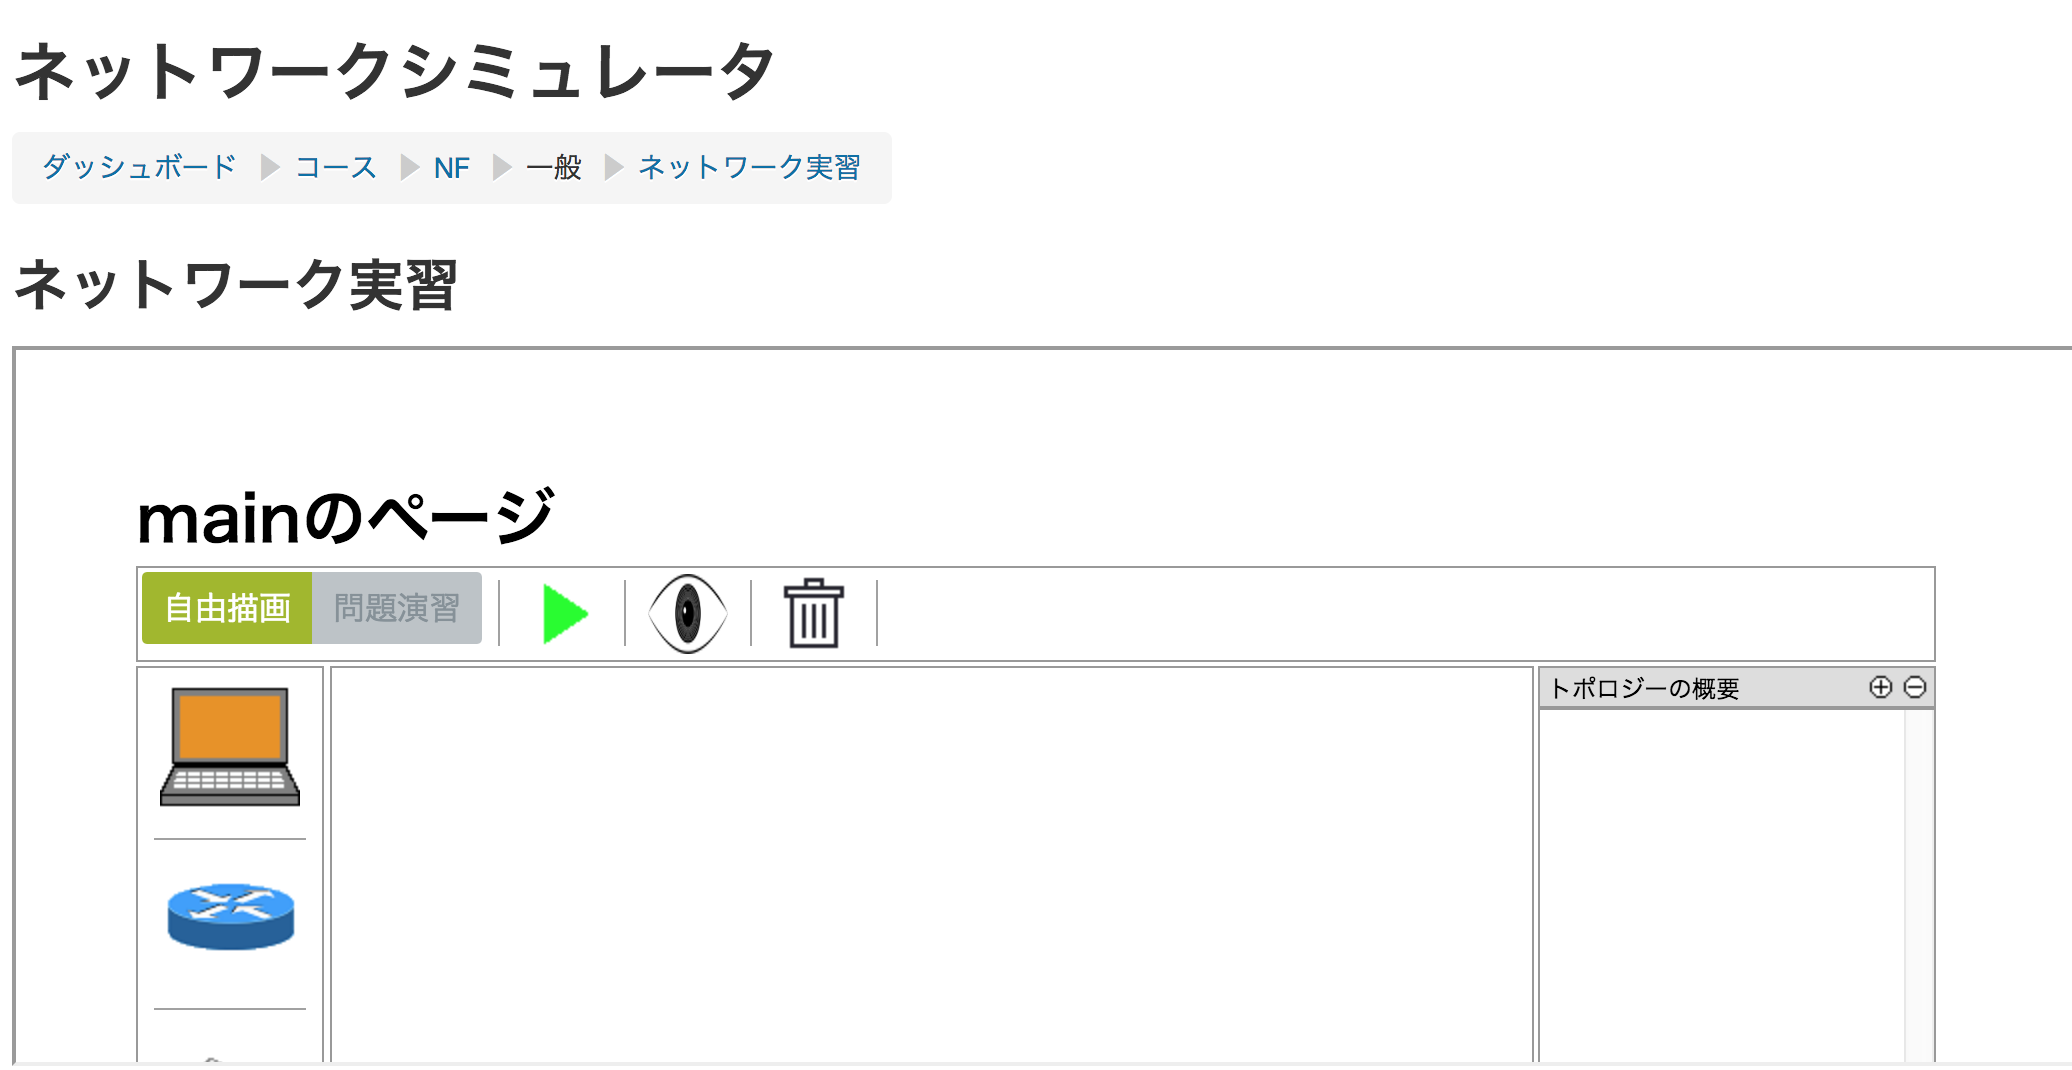
\includegraphics[scale=0.2]{img/LTIstart.png}
    \caption{moodle 外部ツール起動}
    \label{fig:moodle kidou}
  \end{center}
\end{figure}

ユーザとツールコンシューマ間では、ユーザーIDとPWを用いて認証を行う。しかし、ユーザーがツールコンシューマでツールプロバイダを使用する際は、IDとPWを再度入力せずに使用することができる。\\
これがLTIの利点であり、この認証を省くためにOAuthと呼ばれるプロトコルが使われている。
\subsection{OAuth}
OAuth(オーオース)とは、SNSやWebサービス間で「アクセス権限の認可」を行うためのプロトコルである。また、OAuthには1.0と2.0が存在しているが、本研究ではLTI1.0の実装にあたりOAuth1.0を使用している。
\subsection{LTI1.0におけるOAuth1.0実装手順}
OAuth1.0実装にあたり、第三者による不正なログインを防ぐためのOAuth signature(署名)及びkey(暗号)の作成をする関数をRubyで自作した。\\
署名及び暗号の作成手順を以下に示す。\\
1.「キー」を作成\\
2.「文字列」の作成\\
3.「キー」と「文字列」用いて署名を作成\\
\subsubsection{キーの作成}
「oauth\_consumer\_secret」、「oauth\_token\_secret」をURLエンコードし、&で繋げれば完成。\\
本研究では「oauth\_consumer\_secret」を設定し、「oauth\_token\_secret」は存在させなかった。また、各々をURLエンコードし、「oauth token secret」を空白とし、\&のみを繋げてKeyを作成した。
\subsubsection{文字列の作成}
1.パラメータをアルファベット順に並べ、キー=値...の形で並べた上で,URLエンコードする。\\
2.リクエストメソッド、リクエストURLをURLエンコードする。\\
3.リクエストメソッド、リクエストURL、パラメータの順で\&で繋げることで文字列を作成した。\\
\subsubsection{署名の作成}
1.LTI1.0ではHMAC-SHA1方式を採用しているため、作成した「キー」と「署名」を用いてHMAC-SHA1方式でハッシュ値を生成する。この時バイナリデータでハッシュ値を生成する必要がある。\\
2.生成したハッシュ値を、base64エンコードすることで署名を作成。\\
\subsection{成績反映}
成績反映の手順を以下に示す。\\
ツール・コンシューマから成績を返すパラメータ「lis\_outcome\_service\_url」を設定し、特定のユーザーを一意的に示す、「SourcedId」をパラメータ「lis\_result\_sourcedid」から取得し、XML内の「SourcedId」を書き変え、ツール・プロバイダでまとめた点数をXML内の「textString」に加えた上で送信。\\
